\section{General overview}

Figure \ref{fig:switch_top} shows the internals of the WR Switch HDL
design. It contains numerous modules connected with the Wishbone Crossbar.
Each of them has a Wishbone Slave interface and a number of configuration
registers that are read/written from main CPU through the CPU EBI/WB bridge (WB
Master interface). Table \ref{tab:gov:wb_base} contains Wishbone base address of
each module. Blue arrows
in figure \ref{fig:switch_top} represent WR Frabric interface connections
responsible for carrying Ethernet frames between the Endpoints, Switching Core
and Network Interface \linebreak Controller.

\begin{figure}[ht]
  \begin{center}
    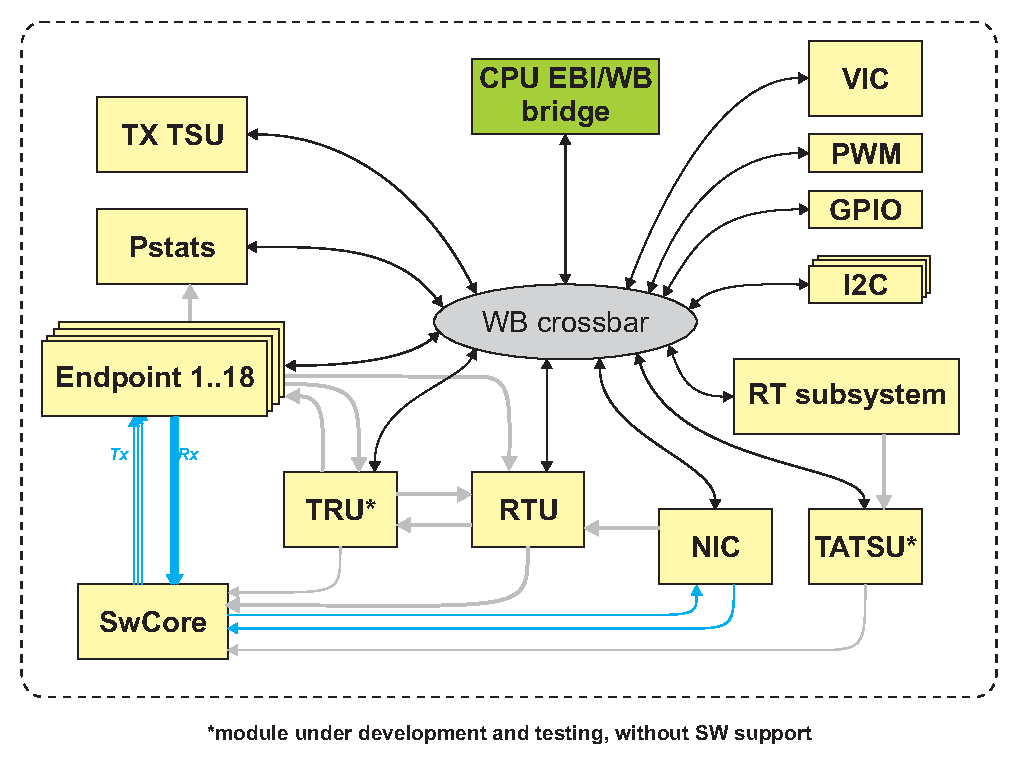
\includegraphics[width=\textwidth]{../../../../figures/switch/switch_hdl_v4.0.ps}
    \caption{Top HDL design of the WR Switch}
    \label{fig:switch_top}
  \end{center}
\end{figure}

\begin{table}
  \begin{center}
  \begin{tabular}{|l|l|}
    \hline
    module name & base address\\
    \hline \hline
    Real-Time subsystem & 0x00000\\
    Network Interface Controller (NIC) & 0x20000\\
    Endpoint fanout & 0x30000\\
    Vectored Interrupt Controller (VIC) & 0x50000\\
    Tx Timestamping Unit (TX TSU) & 0x51000\\
    GPIO port (GPIO)  & 0x53000\\
    $I^2C$ master (I2C0, I2C1, Sensors\_I2C) & 0x54000\\
    PWM Controller & 0x55000\\
    Topology Resolution Unit (TRU) & 0x56000\\
    Time-Aware Traffic Shapper Unit (TATSU) & 0x57000\\
    Per-port Statistics (Pstats) & 0x58000\\
    Hardware Info Unit (HWIU) & 0x59000\\
    Routing Table Unit (RTU) & 0x60000\\
    \hline
  \end{tabular}
  \caption{Wishbone base addresses of modules inside WR Switch HDL}
  \label{tab:gov:wb_base}
  \end{center}
\end{table}
